\chapter{Una panoramica sugli strumenti esistenti}

\section{Selenium}

Selenium \footnote{\url{http://seleniumhq.org}}  sembra essere il sistema più diffuso per l'automazione di test su applicazioni web, grazie alla sua compatibilità con differenti browser e sistemi operativi.
Il progetto si divide in due componenti principali, Selenium IDE e Selenium WebDriver, che hanno funzionalità ben distinte e complementari. 

Selenium IDE è un'estensione per il browser Firefox che permette di registrare e di riprodurre una serie di operazioni su pagine web, specificando anche delle \emph{assertion}, ossia delle verifiche da effettuare durante l'esecuzione del test. Attraverso questo strumento è quindi possibile verificare se la pagina contiene un certo testo in una data posizione nel DOM, o verifiche simili. I test registrati attraverso Selenium possono infine essere esportati in diversi linguaggi ed essere così utilizzati e riadattati all'interno dei framework di test più diffusi, come JUnit, RSpec, PhpUnit, ed altri.

Selenium Webdriver consiste invece in un'interfaccia comune utilizzabile per pilotare i browser più diffusi (Firefox, Internet Explorer, Chrome, Safari e alcuni altri). Attraverso questa interfaccia, è possibile automatizzare l'esecuzione dei test su più browser in parallelo, per verificare il corretto funzionamento dell'applicazione web sui maggiori browser e per velocizzare i tempi di esecuzione dei test.

Di seguito viene presentata un'analisi più dettagliata su ciascuno dei componenti appena descritti.

\subsection{Selenium IDE}

Selenium IDE viene installato come estensione per Firefox,  ed è perciò utilizzabile su tutti i sistemi operativi che supportano questo browser. Stabilito un url di partenza, l'estensione permette di registrare automaticamente una sequenza di operazioni effettuate all'interno delle pagine visualizzate nel browser. 

I click sui collegamenti ipertestuali e sui bottoni di invio dei form, l'inserimento di testo nelle caselle ed altri eventi simili sono intercettati attraverso del codice Javascript iniettato dall'estensione all'interno della pagina, sfruttando il meccanismo di propagazione degli eventi nel DOM. Attraverso Javascript è poi possibile riprodurre programmaticamente gli eventi registrati, simulando così il comportamento dell'utente.

Uno dei problemi principali che si incontrano durante la registrazione automatica è rappresentato dalla scelta del metodo per identificare gli elementi del DOM interessati dagli eventi. Selenium propone diverse alternative, in base alla tipologia di elemento da individuare. Se si tratta di un collegamento ipertestuale, viene utilizzato il testo contenuto nel tag anchor per identificarlo. Se si tratta di un elemento di input, viene scelto invece l'attributo name assegnato al tag. Per tutti gli altri casi, viene infine utilizzato un selettore XPath, meno flessibile ma più specifico.

Se si vuole avere un controllo maggiore sulle azioni da eseguire, è possibile specificarle manualmente anziché eseguirle direttamente sulla pagina corrente. Selenium mette a disposizione un corposo insieme di comandi tra cui scegliere, che simulano anche azioni più complesse come il click con il tasto destro del mouse, lo spostamento del mouse su un elemento, il drag and drop, la pressione di un tasto della tastiera, e simili. E' possibile anche effettuare alcune operazioni sui cookie disponibili per la richiesta corrente, come aggiungerne e modificarne valori. Come specificato prima, ognuno degli eventi simulabili viene riprodotto tramite gli eventi che l'API di Javascript mette a disposizione. 

Oltre alle normali azioni, è possibile specificare attraverso l'IDE anche due tipologie di test, che verranno effettuate durante la riproduzione, nell'ordine cronologico in cui essi sono stati specificati. Le azioni di tipo \emph{assert} controllano che i criteri definiti siano rispettati e se ciò non avviene interrompono l'esecuzione del test. Le azioni di tipo \emph{verify} invece svolgono lo stesso compito, ma non interrompono il flusso di esecuzione nel caso in cui una verifica fallisca.
Alcuni dei comandi di test più comuni consentono poi di verificare che un elemento della pagina specificato da un selettore contenga un determinato testo, che un elemento abbia certe dimensioni o una certa posizione assoluta, che una certa opzione in un menù a tendina sia selezionata, e così via. Altri comandi più sofisticati verificano il numero di elementi di un certo tipo presenti sulla pagina, la loro visibilità, il contenuto dei cookie impostati.

\begin{figure}[htbp]
\begin{center}
\includegraphics[width=\textwidth]{images/selenium_screen.png}
\caption{Interfaccia dell'estensione Selenium IDE}
\label{fig:selenumScreen}
\end{center}
\end{figure}

Sia per le azioni specificate manualmente, sia per le verifiche, è necessario specificare il \emph{target}, ossia l'elemento nel DOM (o gli elementi) interessati. Per far ciò, chi scrive il test deve inserire manualmente un selettore CSS o XPath, in quanto l'estensione non fornisce strumenti di supporto per questo compito. A tale scopo è necessario esaminare manualmente il DOM della pagina e ricavare il selettore che si ritiene più indicato. Sarà quindi responsabilità completa dello sviluppatore la scelta di un selettore sufficientemente flessibile nel caso di cambiamenti approntati in un secondo momento alla struttura della pagina, come l'aggiunta di nuovi elementi, la modifica degli attributi di classe, eccetera. 

Dopo che è stata registrata una serie di azioni e di verifiche, è possibile salvarla in formato HTML, sotto forma di tabella, con una colonna per il comando Selenium da eseguire, una per il target del comando e una per i parametri aggiuntivi da passare al comando. Questo tipo di formattazione tabellare dei test è ispirata a quella utilizzata nel framework di test Fitness \footnote{\url{http://fitnesse.org}}.

Più interessante è la possibilità di esportare il test case registrato in uno dei linguaggi supportati, tra i quali Php, Ruby, Python, Java e C\#. I comandi specificati tramite l'IDE saranno in questo modo tradotti in istruzioni per il componente WebDriver, descritto nella prossima sezione. Gli stessi sviluppatori di Selenium suggeriscono di utilizzare l'estensione per Firefox come un punto di partenza nella creazione di test case, e di raffinare le azioni registrate e le verifiche da effettuare dopo la traduzione in un linguaggio che utilizzi WebDriver.

\subsection{Selenium WebDriver}

Selenium WebDriver è stato rilasciato a Luglio del 2011 \footnote{\url{http://seleniumhq.wordpress.com/2011/07/08/selenium-2-0}}, in concomitanza con il rilascio della versione 2.0 di Selenium, che ha introdotto notevoli novità rispetto al passato.
WebDriver è nato come progetto indipendente e nell'Agosto 2009 gli sviluppatori hanno deciso di unire gli sforzi ed i risultati ottenuti con il team di sviluppo di Selenium RC.

WebDriver nasce come un'insieme di binding per pilotare differenti browser attraverso un insieme di linguaggi. Per controllare i browser al fine di simulare l'azione dell'utente, il progetto si interfaccia con le istanze dei browser attraverso un protocollo in stile RPC, chiamato \emph{Wire protocol} \footnote{\url{http://code.google.com/p/selenium/wiki/JsonWireProtocol}} , che prevede l'invio di comandi in stile HTTP su di un socket locale. 

Tale meccanismo permette la comunicazione diretta tra il processo del browser e il processo del programma che esegue il test (chiamato Client). I comandi ed i relativi parametri vengono serializzati in formato JSON e il formato con il quale essi sono definiti si basa sul paradigma REST, come descritto in \cite{architectureOfOpenSource}. 

A seconda del browser, vengono utilizzate strategie diverse per riuscire a comunicare con il browser attraverso il protocollo Wire: se ad esempio si vuole utilizzare il browser Firefox è necessario installare un'apposita estensione che interpreta i comandi del protocollo e li traduce in chiamate all'interfaccia nativa messa a disposizione dal browser, secondo l'architettura mostrata in figura ~\ref{fig:webdriverFirefox}.

\begin{figure}[htbp]
\begin{center}
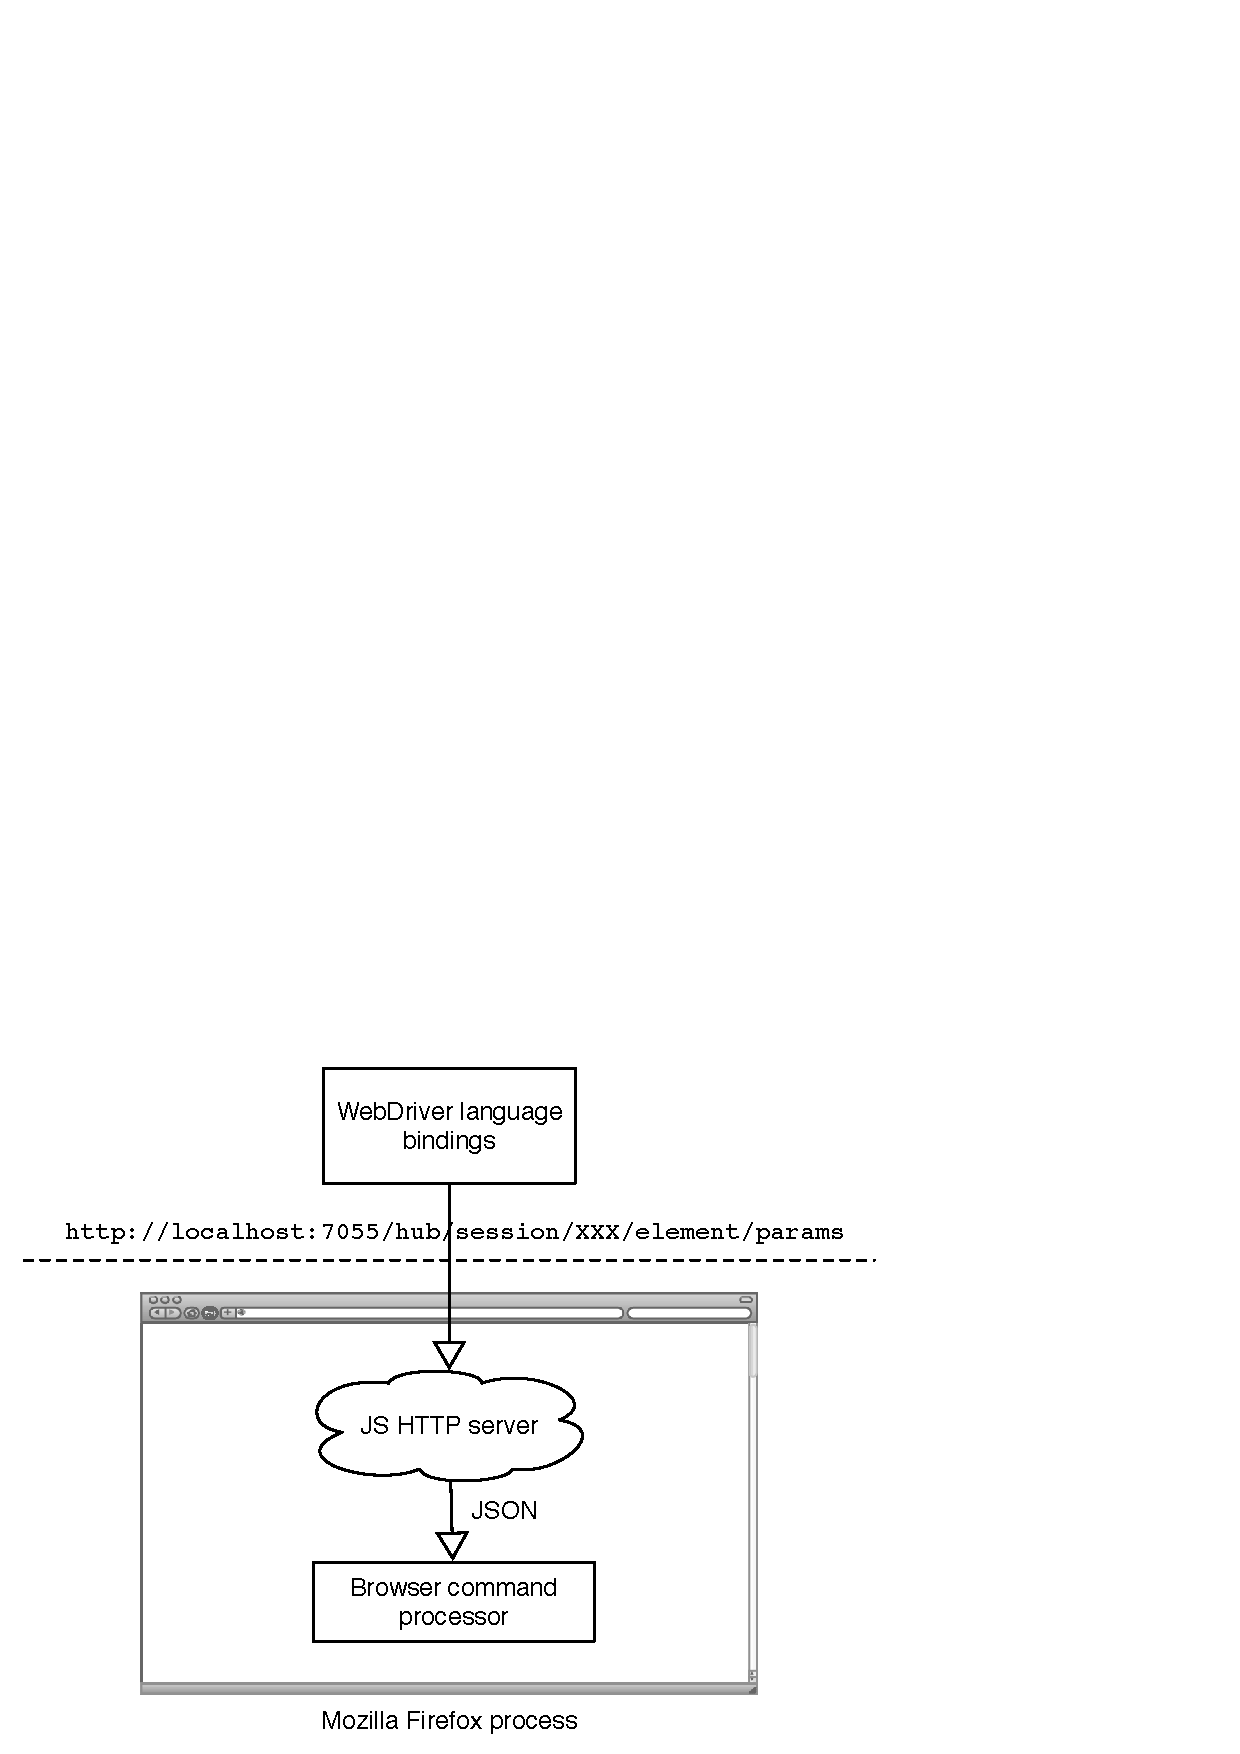
\includegraphics[width=\textwidth]{images/webdriver_firefox.png}
\caption{Architettura del protocollo Wire per il FirefoxDriver}
\label{fig:webdriverFirefox}
\end{center}
\end{figure} 

Attualmente, WebDriver fornisce il codice per pilotare Firefox, Internet Explorer, Chrome, Safari, Opera e Android Browser. In aggiunta, è possibile utilizzare il driver per HtmlUnit, un'implementazione interamente in memoria di un browser che non si occupa di mostrare visivamente il contenuto delle pagine web. Questa opzione è utile per simulare gli scenari più semplici in maniera molto veloce, poiché si evita l'overhead dovuto alla visualizzazione grafica delle pagine. 
Il team di Selenium sta collaborando attivamente con gli sviluppatori di questi browser per incorporare la gestione del protocollo Wire all'interno del browser stesso, migliorandone la possibilità di essere pilotato dall'esterno. 

I vantaggi di questo sistema sono molteplici. In primo luogo, è possibile effettuare test automatizzati su differenti browser, assicurandosi che l'applicazione web in esame funzioni correttamente nella maggior parte delle modalità d'uso da parte dell'utente finale. 

In secondo luogo, il browser viene pilotato nativamente, senza bisogno di ricorrere all'esecuzione di codice javascript per intercettare e simulare gli eventi. Questo innalza il livello di accuratezza della simulazione e permette di superare alcuni limiti di sicurezza imposti dall'interprete del codice javascript implementato nel browser, in particolare riguardo alla \emph{same origin policy} (\cite{sameOrigin}) e di accedere ad alcune informazioni e funzionalità avanzate normalmente non accessibili tramite codice javascript.

Inoltre, l'implementazione dei Driver è slegata da quella dei Client, che possono essere quindi scritti in un qualsiasi linguaggio che fornisca primitive per inviare dati su di un socket. Ciò permette di scrivere i test veri e propri nel linguaggio con cui si hanno più confidenza e competenze. Selenium mette a disposizione client già pronti sotto forma di librerie nei maggiori linguaggi di scripting, come Php, Ruby e Python, oltre che in Java e C\#.

Come svantaggi, il sistema è molto completo ma rischia di risultare decisamente complicato e difficile da mantenere, utilizzando componenti basati su tecnologie molto diverse tra loro. Dal punto di vista dell'utilizzatore, il sistema di per sé non offre alcun supporto o automazione nella scrittura dei test veri e propri. 

\section{Windmill}

Il progetto open source Windmill \footnote{\url{http://www.getwindmill.com}} permette di effettuare il testing di interfacce web su differenti browser, simulando il comportamento dell'utente attraverso codice javascript iniettato nelle pagine. Il software è scritto in Python e viene eseguito da linea di comando. Il browser scelto per eseguire i test viene lanciato da linea di comando, viene impostato un profilo di utilizzo comprensivo delle estensioni necessarie e viene configurato come proxy del browser il server HTTP di Windmill, il quale di occupa di interagire con le pagine. 

\begin{figure}[htbp]
\begin{center}
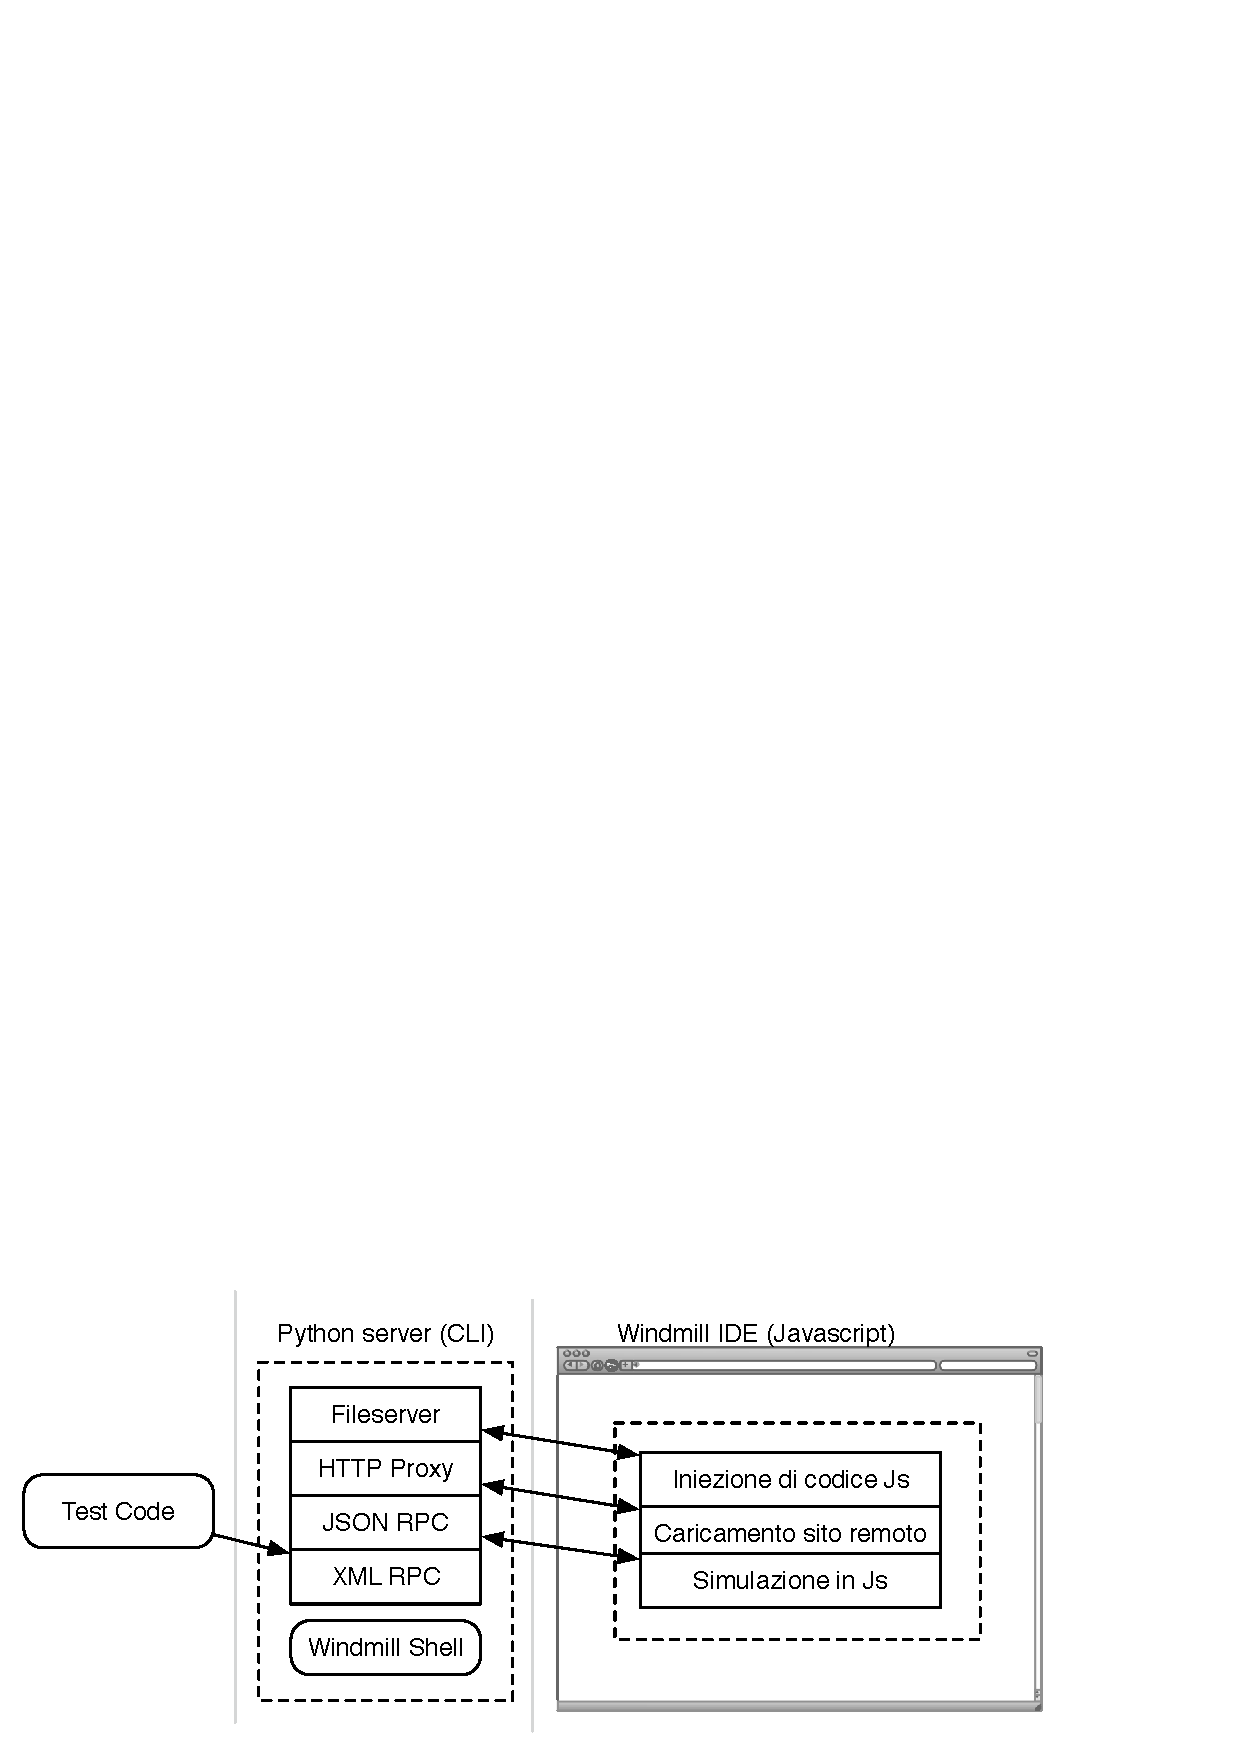
\includegraphics[width=\textwidth]{images/windmill_architecture.png}
\caption{Architettura di Windmill}
\label{fig:windmillArchitecture}
\end{center}
\end{figure}

L'architettura generica di questo progetto è mostrata in figura ~\ref{fig:windmillArchitecture}. La strategia utilizzata è molto simile a quella riscontrata in Selenium RC, componente del progetto che è stato deprecato con il rilascio della versione 2 in favore di WebDriver. 

Il componente principale di Windmill è il servizio realizzato in Python. I test possono essere definiti in un qualunque linguaggio che sia in grado di effettuare richieste HTTP, poiché la comunicazione tra il linguaggio in cui sono definiti i test ed il server in Python incluso nel servizio avviene tramite protocollo XML RPC. Il server infatti espone ai client una serie di funzioni richiamabili tramite richieste HTTP.

I comandi possono anche essere invocati direttamente in una shell integrata ed è così possibile interagire in tempo reale con il browser.

Il servizio si occupa poi di lanciare le istanze dei browser supportati con i parametri necessari a stabilire l'ambiente di test. Il browser Firefox ad esempio viene lanciato utilizzando un profilo speciale definito da Windmill, che evita di dover caricare estensioni aggiuntive che potrebbero interferire con i test. Inoltre, il server HTTP in Python viene impostato come proxy server per il browser.

L'uso del proxy server consente di pilotare il browser richiamando il codice Javascript per simulare gli eventi che viene iniettato nelle pagine web. La comunicazione avviene tramite protocollo JSON RPC.

La libreria javascript iniettata deve uniformare le diverse implementazioni dell'interprete javascript per i browser supportati, in modo da poter simulare gli stessi eventi in ognuno dei browser. 

Oltre che dalla shell interattiva di Python, è possibile registrare direttamente i test sulle pagine web visualizzate nel browser utilizzando un' interfaccia per Windmill, che si apre in una finestra separata del browser ed è realizzata come una semplice pagina web.

\begin{figure}[htbp]
\begin{center}
\includegraphics[width=\textwidth]{images/windmill_screen.png}
\caption{Interfaccia in HTML e Javascript di Windmill}
\label{fig:windmillScreen}
\end{center}
\end{figure}

Attraverso l'interfaccia è possibile registrare le azioni che si stanno eseguendo sulla pagina e rieseguirle, in maniera simile a quanto è possibile fare attraverso Selenium IDE. Per identificare gli elementi interessati dagli eventi e dalle assertion, vengono utilizzati automaticamente selettori XPath. E' possiible poi agire manualmente e utilizzare un selettore CSS o altri attributi dei tag HTML. Per selezionare l'elemento da verificare, viene messo a disposizione un DOM inspector che evidenzia gli elementi del DOM al passaggio del mouse sulla pagina e al click sul nodo seleziona il percorso XPath per identificarlo.

Da segnalare anche la possibilità di scrivere manualmente i test in Javascript, utilizzando la libreria apposita del progetto, oppure in Python, e di integrare Windmill all'interno del framework Django per applicazioni web in Python.

Il progetto è mantenuto attivamente dagli sviluppatori, ma la documentazione risulta abbastanza scarna. %TODO completare?

\section{Watir}

Watir consiste in un insieme di librerie in Ruby per automatizzare l'uso dei principali browser, ossia Chrome, Firefox, Opera, Safari, Internet Explorer. I test per l'applicazione interessata vengono scritti in maniera programmatica ed è possibile integrare l'uso di Watir in alcuni dei framework di testing per Ruby più utilizzati, come RSpec o Test::Unit, attraverso i quali è possibile gestire la definizione, l'esecuzione e la generazione di report dei test.

Watir espone allo sviluppatore un insieme di metodi molto flessibili e allo stesso tempo concisi e di facile utilizzo, grazie soprattutto alla potenza espressiva del linguaggio Ruby. E' possibile pilotare il browser eseguendo tutte le azioni di interesse per un test di una applicazione web, come la compilazione di form, la navigazione attraverso i collegamenti, la pressione di pulsanti e il click su altri elementi. 

Per accedere agli elementi del DOM, si utilizzano apposite collezioni fornite dal framework, corredate di metodi che ne facilitano le operazioni comuni. Da questo punto di vista, rispetto alle librerie simili, Watir offre dalla versione 2.0 la possibilità aggiuntiva di utilizzare criteri multipli per la selezione di nodi del DOM: è possibile infatti accedere ad un elemento combinando ad esempio due condizioni, una sull'attributo \emph{name} e una sull'attributo \emph{class} del tag HTML. Come ci si aspetta, è inoltre possibile utilizzare selettori CSS o XPath.

Sotto il profilo tecnico, per pilotare i browser Watir utilizza i binding in Ruby di WebDriver, già visto in precedenza come parte integrante di Selenium. Di fatto quindi Watir consiste semplicemente in un wrapper per WebDriver, che però ne rende l'uso molto più agevole. Prima dell'esecuzione del test, il browser scelto viene lanciato tramite linea di comando, utilizzando un profilo d'uso apposito che non contiene estensioni o plugin abilitati. Siccome vengono utilizzati internamente i driver di WebDriver, la simulazione utilizza eventi nativi del browser, assicurando una notevole accuratezza anche nell'esecuzione di codice Javascript presente nell'applicazione sotto esame. Nel caso specifico di Internet Explorer, Watir implementa direttamente una libreria che permette di interagire su sistema Windows con tale browser utilizzando la tecnologia Microsoft COM per realizzare la comunicazione tra differenti processi in esecuzione.

E' utile infine segnalare per completezza che fino alla versione 1.X Watir utilizzava l'estensione JSSh per pilotare i browser Mozilla. Essa consiste in un modulo binario realizzato in C++ che consente di stabilire una connessione TCP/IP verso un processo Mozilla in esecuzione. Una volta stabilita la connessione, si utilizza una sorta di shell con comandi Javascript per controllare in maniera remota il browser. L'estensione JSSh può essere considerata come un prototipo del più moderno protocollo Wire, di cui si è trattato in precedenza. Dalla versione 4 di Firefox però JSSh è stata abbandonata e Watir utilizza attualmente il driver per Firefox presente nelle librerie WebDriver.


%\lstset{basicstyle=\ttfamily, breaklines=true, language=Ruby, tabsize=2, caption=Descriptive Caption Text, numbers=left, stepnumber=2, frame=single}
%TODO: descrivere sincronizzazione ajax con watir?

\lstinputlisting[float=h, caption=Esempio di utilizzo di Watir e RSpec ]{code/watir_example.rb}


%\section{Sahi}
